\documentclass[a4paper]{scrreprt}

\usepackage[german]{babel}
\usepackage[utf8]{inputenc}
\usepackage[T1]{fontenc}
\usepackage{ae}
\usepackage{amssymb}
\usepackage{graphicx}
\usepackage{hyperref}

\begin{document}

m\title{BS Zusammenfassung}
\author{Benedict Hauck, Fedor Scholz}
\maketitle

\tableofcontents
\vspace{1cm}

\chapter{01aIntro}

\section{Was ist ein Betriebssystem?}
\begin{itemize}
	\item Vermittler zwischen Benutzer und Computer
	\item Ziele
		\begin{itemize}
			\item Benutzerprogramme ausfuehren und dem Benutzer das Loesen von Problemen erleichtern
			\item Computer benutzbarer machen
			\item Hardware des Computer effizient nutzen
		\end{itemize}
	\item Vier Komponenten eines Computersystems
		\begin{itemize}
			\item Benutzer
			\item System- und Anwendungsprogramme
			\item Betriebssystem
			\item Hardware
		\end{itemize}
	\item Betriebssysteme verteilen Ressourcen
		\begin{itemize}
			\item Verwaltung aller Ressourcen
			\item Entscheidung bei konfligierenden Anfragen fuer effizientes und faires Benutzen der Ressourcen
		\end{itemize}
	\item Betriebssysteme kontrollieren
		\begin{itemize}
			\item Kontrolle von Ausfuehrungen von Programmen um Fehler und ungeeignetes Benutzen des Computers zu verhindern
		\end{itemize}
	\item Immer laufendes Programm ist Kernel, Rest ist System- oder Anwendungsprogramm
	\item Bootstrap program wird beim Starten oder Neustarten geladen
		\begin{itemize}
			\item In ROM, EPROM oder FLASH als firmware gespeichert
			\item Initialisiert alle Aspekte des Systems, insbesondere die HW-Komponenten
			\item Laedt den Kernel und startet die Ausfuehrung
		\end{itemize}
\end{itemize}

\section{Organisation}
\begin{itemize}
	\item Ein oder mehr CPUs, device controllers verbinden sich ueber den Bus um Zugriff auf shared memory zu bekommen
	\item I/O-Geraete und CPU koennen gleichzeitig ausfuehren
	\item Jeder device controller ist zustaendig fuer einen Geraetetypen
	\item Jeder device controller hat einen lokalen Puffer
	\item CPU bewegt Daten vom/zum Hauptspeicher zu/von lokalen Puffern
	\item I/O ist vom Geraet zum lokalen Puffer des controllers
	\item device controller informiert CPU per interrupts, wenn er fertig ist
\end{itemize}


\section{Interrupts}
\subsection{Haeufige Funktionen von Interrupts}
\begin{itemize}
	\item interrupt gibt Kontrolle an interrupt service routine ueber einen interrupt vector, welcher die Adressen von allen service routines beinhaltet
	\item interrupt architecture muss Adresse der unterbrochenen Intruktion speichern
	\item Einkommende interrupts sind aus, wenn gerade ein anderer bearbeitet wird um lost interrupts zu verhindern
	\item trap ist ein interrupt, welcher von Software verursacht wurde (wegen eines Fehler oder durch eine Benutzeranfrage)
	\item Betriebssysteme sind interrupt driven
\end{itemize}

\subsection{Timer interrupts}
\begin{itemize}
	\item Time interrupts um endlose Schleifen und Prozesse zu verhindern
	\item Wird nach bestimmter Zeitspanne ausgefuehrt
	\item Wird vor dem schedulen des Programm aufgesetzt
	\item Eingebettete Systeme haben Watchdog, welche bis 0 zaehlt und dann resettet
\end{itemize}

\subsection{Interrupt Handling}
\begin{itemize}
	\item Betriebssystem merkt sich Status der CPU, indem es Register und Programmzaehler speichert
	\item Legt Typ des interrupts fest
		\begin{itemize}
			\item polling
			\item vectored interrupt system
		\end{itemize}
\end{itemize}

\section{I/O Struktur}
\subsection{Synchrone oder blockende I/O}
\begin{itemize}
	\item Nachdem I/O beginnt, geht die Kontrolle erst nach Fertigstellung der I/O wieder zum Benutzerprogramm
	\item Wait instruction laesst die CPU idlen
	\item Meistens nur ein I/O Request gleichzeitig
	\item Polling
	\item Signal
	\item Callback function
\end{itemize}

\subsection{Direct Memory Access Structure}
\begin{itemize}
	\item Fuer high-speed I/O, damit diese mit fast der Geschwindigkeit des Hauptspeichers Informationen uebertragen koennen
	\item Device Controller uebertraegt Daten in Bloecken vom Puffer direkt in den Hauptspeicher ohne CPU Eingriff
	\item Nur ein interrupt pro Block
\end{itemize}

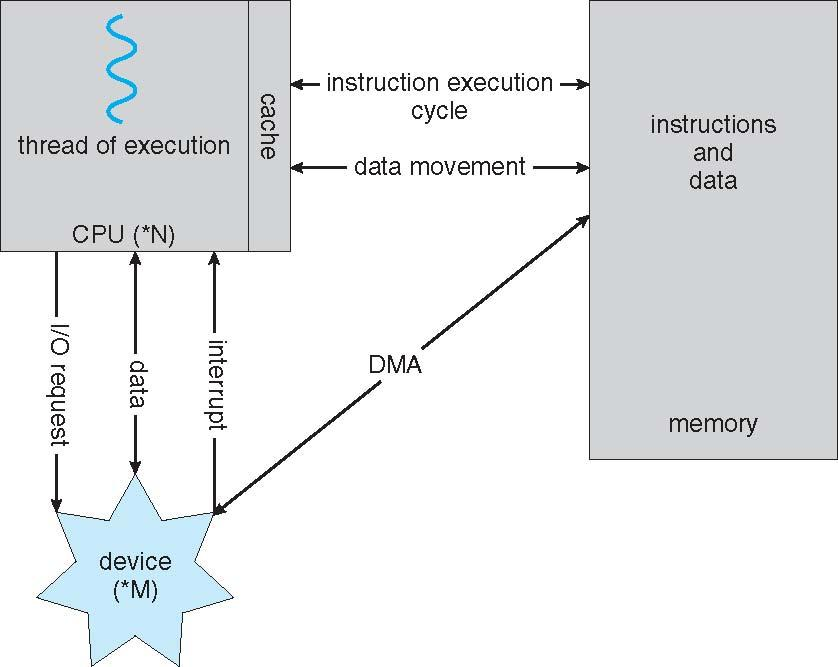
\includegraphics[scale=0.4]{dma.png}

\section{Computer-System Architektur}
\subsection{Multiprozessor-Systeme}
\begin{itemize}
	\item Auch parallel systems, tightly-coupled systems
	\item Vorteile
		\begin{itemize}
			\item Erhoehter Durchsatz
			\item Wirtschaftlichkeit durch große Serie
			\item Erhoehte Zuverlaessigkeit - Fehlertoleranz
		\end{itemize}
	\item Zwei Typen
		\begin{itemize}
			\item Asymmetrische Mehrfachprozessorarchitektur
			\item Symmetrische Mehrfachprozessorarchitektur
		\end{itemize}
	\item Typen von Multiprozessoren
		\begin{itemize}
			\item Multi-socket systems
			\item Multi-Chip Module (MCM) (=Multi-Core)
			\item Chip Multiprocessor (CMP) (=Multi-Core)
			\item Simultaneous MultiThreading Processor (SMT)
		\end{itemize}
\end{itemize}

\subsection{Geclusterte Systeme}
Wie Multiprozessorsystem, nur dass mehrere Systeme zusammen arbeiten

\begin{itemize}
	\item Teilen sich meistens Speicher ueber storage-area network (SAN)
	\item Ermoeglicht hochverfuegbare Services, welche Fehler ueberleben
		\begin{itemize}
			\item Asymmetrisches Clustern hat eine Maschine im hot-standby mode
			\item Symmetrisches Clustern hat viele Maschinen mit laufenden Programmen, welche sich gegenseitig beobachten
			\item Manche sind fuer hochperfomantes computing (HPC)
		\end{itemize}
\end{itemize}

\section{Betriebssystem Struktur}
\begin{itemize}
	\item Multiprogramming ist noetig fuer Effizienz
		\begin{itemize}
			\item Einzelner Benutzer kann nicht CPU und I/O die ganze Zeit auslasten
			\item Multiprogramming organisiert jobs, sodass CPU immer beschaeftigt ist
			\item Untermenge aller Jobs ist im Hauptspeicher
			\item Einer wird ausgewaehlt per job scheduling
			\item Wenn dieser warten muss, wechselt OS den job
		\end{itemize}
	\item Timesharing (multitasking) laesst CPU so schnell jobs wechseln, sodass interaktives computing moeglich ist
		\begin{itemize}
			\item Response time < 1 Sekunde
			\item Jeder Benutzer hat mindestens 1 Programm im Speicher, welches ausgefuehrt wird $\Rightarrow$ process
			\item Wenn mehrere jobs bereit sind $\Rightarrow$ CPU scheduling
			\item Wenn Prozess nicht in Speicher passt $\Rightarrow$ swapping
			\item Virtueller Speicher erlaubt Ausfuehrung von Prozessen nicht komplett im Speicher
		\end{itemize}
\end{itemize}

\section{Uebergang vom User zum Kernel Mode}
\begin{itemize}
	\item Interrupt gesteuert durch Hardware
	\item Softwarefehler oder Anfrage erzeugt exception oder trap
	\item Dual-mode erlaubt es OS, sich und andere Komponenten zu schuetzen
	\item Mode bit bereitgestellt durch HW
		\begin{itemize}
			\item Zeigt an, ob System im User oder Kernel Mode ist
			\item Manche previligierten Instruktionen sind nur im Kernel Mode moeglich
			\item System call aendert Modus zu Kernel, Wiederkehr vom call aender Modus zu User
		\end{itemize}
\end{itemize}

\section{Prozessverwaltung}
\begin{itemize}
	\item Prozess ist ein Programm waehrend der Ausfuehrung: Programm ist eine passive, Prozess eine aktive Einheit
	\item Prozessbeedigung erfordert das freigeben von genutzten Ressourcen
	\item Single-threaded process hat einen program counter und wird sequentiell ausgefuehrt
	\item Multi-threaded process hat einen program counter pro thread
	\item Das Betriebssystem ist dabei fuer folgendes zustaendig:
		\begin{itemize}
			\item Erschaffen und loeschen von Benutzer- und Systemprozessen
			\item Suspenden und resumen von Prozessen
			\item Bereitstellung von Mechanismen fuer Prozessynchronisation
			\item Bereitstellung von Mechanismen fuer Prozeskommunikation
			\item Bereitstellung von Mechanismen fuer das Behandeln von deadlocks
		\end{itemize}
\end{itemize}

\section{Speicher}
\subsection{Storage Structure}
\begin{itemize}
	\item Hauptspeicher - großer Speicher, auf welchen CPU direkt zugreifen kann
	\item Zweitspeicher - Erweiterung des Hauptspeichers, welche groß und nicht fluechtig ist
	\item Magnetische Disks - Oberflaeche in tracks geteilt, welche wiederum aus Sektoren bestehen
\end{itemize}

\subsection{Speicherverwaltung}
\begin{itemize}
	\item Alle Daten muessen vor und nach Verarbeitung im Speicher sein
	\item Alle Instruktionen muessen in der Reihenfolge ihrer Ausfuehrung im Speicher sein
	\item Aktivitaeten des OS
		\begin{itemize}
			\item Darauf achten, wer was im Speicher benutzt
			\item Bestimmen, welche Prozesse und Daten in und aus dem Speicher gehen
			\item Zuteilen und freigeben von Speicherplatz
			\item Einheitlichen, logischen Ueberblick bieten
				\begin{itemize}
					\item Abstrahiert physikalischen Eigenschaften zu logischen Einheiten: Dateien
					\item Jedes Medium wird von einem device kontrolliert
				\end{itemize}
		\end{itemize}
	\item Dateisystemverwaltung
		\begin{itemize}
			\item Dateien haeufig in Ordner organisiert
			\item Kontrolle ueber Zugriff
			\item Aktivitaeten des OS
				\begin{itemize}
					\item Erstellen und Loeschen von Dateien und Ordnern
					\item Grundsaetzliche Moeglichkeiten zum manipulieren von Dateien und Ordnern
					\item Abbilden von Dateien in sekundaere Speicher
					\item Sichern von Dateien auf nichtfluechtige Speicher
				\end{itemize}
		\end{itemize}
\end{itemize}

\subsection{Speicherhierarchie}
Die Speicherhierarchie haengt von folgenden Punkten ab:
\begin{itemize}
	\item Geschwindigkeit
	\item Kosten
	\item Fluechtigkeit
\end{itemize}

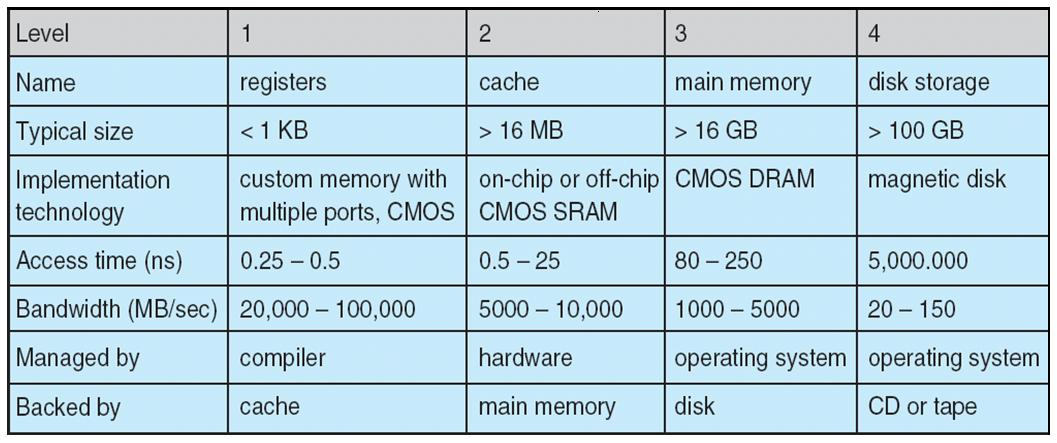
\includegraphics[scale=0.4]{storage.png}

\subsection{Caching}
\begin{itemize}
	\item Wichtiges Prinzip, taucht immer wieder auf (HW, OS, SW)
	\item Benutzte Information wird temporaer von langsameren zu schnelleren Speichern bewegt
	\item Zuerst wird im schnellen Speicher nach Information gesucht
		\begin{itemize}
			\item Wird sie gefunden, wird sie direkt benutzt
			\item Ansonsten wird sie in Cache kopiert und dort benutzt
		\end{itemize}
	\item Cache ist kleiner als Speicher, welcher gecached wird
\end{itemize}





\chapter{01bCProgramming}
\chapter{02OS}

\section{Monolithisches System}
Vorteile:
	\begin{itemize} 
		\item Einfacher Zugriff auf alle Systemdaten 
		\item Kosten von Modulinteraktionen sind niedrig
		\item Erweiterbar über Schnittstellen
		\item Vorhersehbares Verhalten 
	\end{itemize}
Nachteile:
	\begin{itemize}
		\item Kein Schutz zwischen System und Anwendung
		\item Instabil
	\end{itemize}

Beispiele:
	\begin{itemize}
		\item uCLinux, RTOSe, eCos
	\end{itemize}
	
\section{Mehrschichtiger Ansatz}
	\begin{itemize}
		\item Betriebssystem ist in n Schichten aufgeteilt
		\item Jede Schicht kann nur auf die Funktionen und Dienste von niedrigeren Schichten zugreifen 
			\begin{itemize} 
				\item Schicht 0 ist die Hardware
				\item Schicht n ist das Benutzerinterface
			\end{itemize}
		\item Einfachere Migration zwischen Plattformen
		\item Einfachere Evolution der Hardwareplattform
		\item Niedrigere Schichten implementieren Mechanismen
		\item Höhere Schichten implementieren meistens Policies
	\end{itemize}

\begin{center}
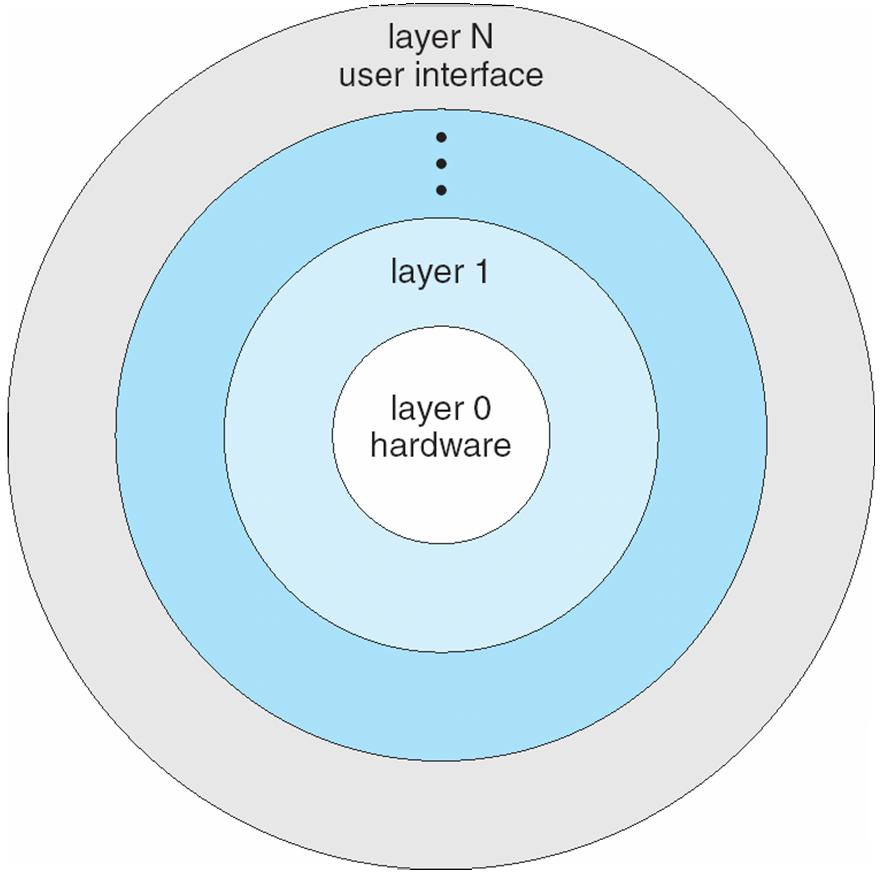
\includegraphics[scale=0.15] {schichtenmodell.png} 
\end{center}

Vorteile:
	\begin{itemize}
		\item Jede Schicht kann unabhängig getestet und verfiziert werden
		\item Korrektheit von Schicht n hängt nur von Schicht n-1 ab (einfacheres Debugging, einfachere Wartung)
	\end{itemize}

Nachteile:
	\begin{itemize}
		\item Nur unidirektionaler Schutz
		\item Beiseitige Abhängigkeit von Schichten verhindert strikte Schichtenbildung
	\end{itemize}
Beispiele:
	\begin{itemize}
		\item THE (Dijkstra), Multics(GE), VOCOS(EWSD)
	\end{itemize}
	
\section{Monolitische Kernels}
	\begin{center}
		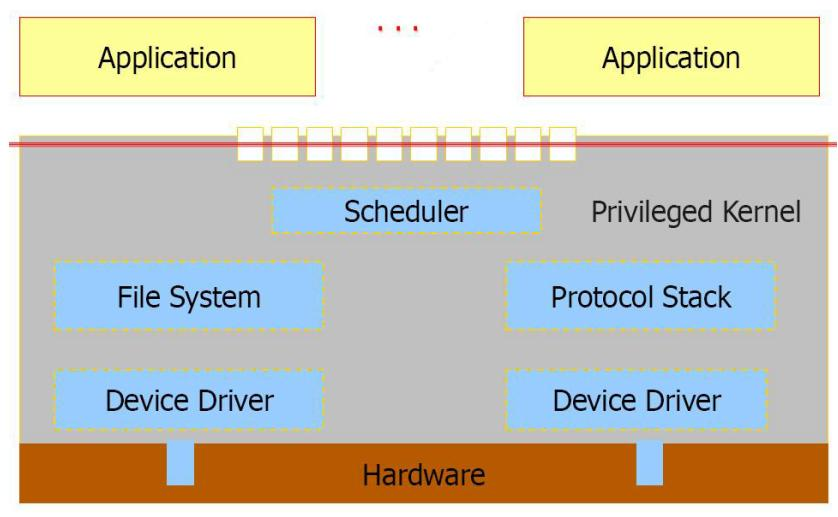
\includegraphics[scale=0.3] {monolithickernel.png}
	\end{center}
	Vorteile:
		\begin{itemize}
			\item "Gute" Performance
			\item Ausreichender Schutz zwischen Anwendungen
			\item Erweiterbar über Schnittstellen und statische/ladbare Module
		\end{itemize}
	Nachteile:
		\begin{itemize}
			\item Kein Schutz zwischen Kernel-Komponenten
			\item Nebeneffekte durch undokumentierte Interfaces
			\item Hohe Komplexität durch hohe gegenseitige Abhängigkeit
		\end{itemize}
	Beispiele
		\begin{itemize}
			\item Linux, Solaris
		\end{itemize}

\section{Microkernel Systeme}
	\begin{center}
		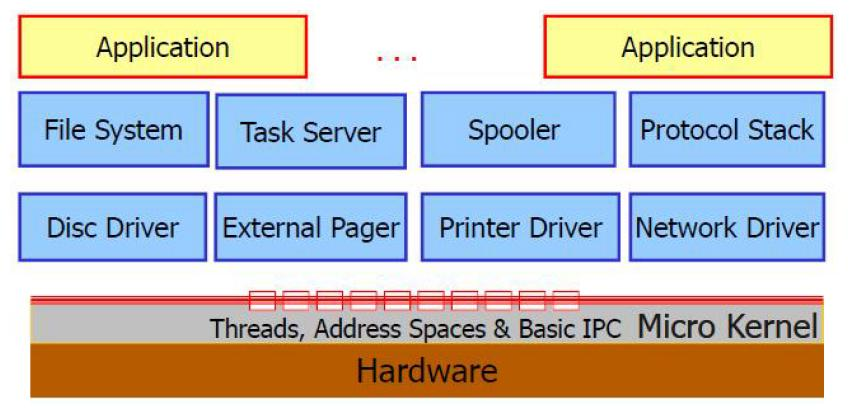
\includegraphics[scale=0.3] {microkernel.png}
	\end{center}

	\begin{itemize}
		\item Möglichst viel des Kernels in den "Benutzer" space packen
		\item Kommunikation erfolgt zwischen Benutzermodulen mit Nachrichtenweitergabe
	\end{itemize}
	
	Vorteile:
		\begin{itemize}
			\item Einfacher einen Microkernel zu erweitern
			\item Einfacher das Betriebssystem auf neue Architekturen zu portieren
			\item Zuverlässiger (es läuft weniger Code im Kernel-Modul
			\item Mehrere APIs vorhanden
			\item Verbesserte Robustheit und Sicherheit
			\item Einfacher zum Testen und Beweisen
			\item Verbesserte Wartbarkeit
		\end{itemize}
	Nachteile:
		\begin{itemize}
			\item Performance Unkosten durch Kommunikation von Benutzerspace zum Kernelspace 
			\item Zusätzliche Zersetzung
			\item Schlechte Erfahrungen mit IBMs Workplace OS (1991-1995)
		\end{itemize}

\section{Virtuelle Maschinen}
	\begin{itemize}
		\item Eine virtuelle Maschine nimmt den mehrschichtigen Ansatz und behandelt Hardware sowie den Kernel des Betriebssystems so als wären sie Hardware
		\item Eine virtuelle Maschine stellt ein identisches Interface zu der blanken, darunterliegenden Hardware
		\item Der Betriebssystem-Host kreiert die Illusion das ein Prozess sein eigenen Prozessor und (virtuellen Speicher) hat.
		\item Jeder Gast bekommt eine Kopie des darunterliegenden Computers zur Verfügung gestellt.
	\end{itemize}
	Vorteile:
		\begin{itemize}
			\item Mehrere Betriebssysteme können sich die gleiche Hardware teilen
			\item Gegenseitiger Schutz
			\item Nützlich für Development und Testen
		\end{itemize}
	\begin{center}
		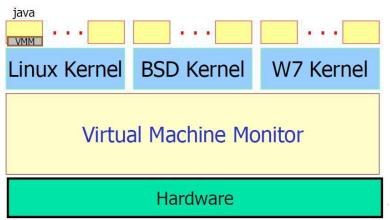
\includegraphics[scale=0.5] {virtualmachine.png}
		\\
		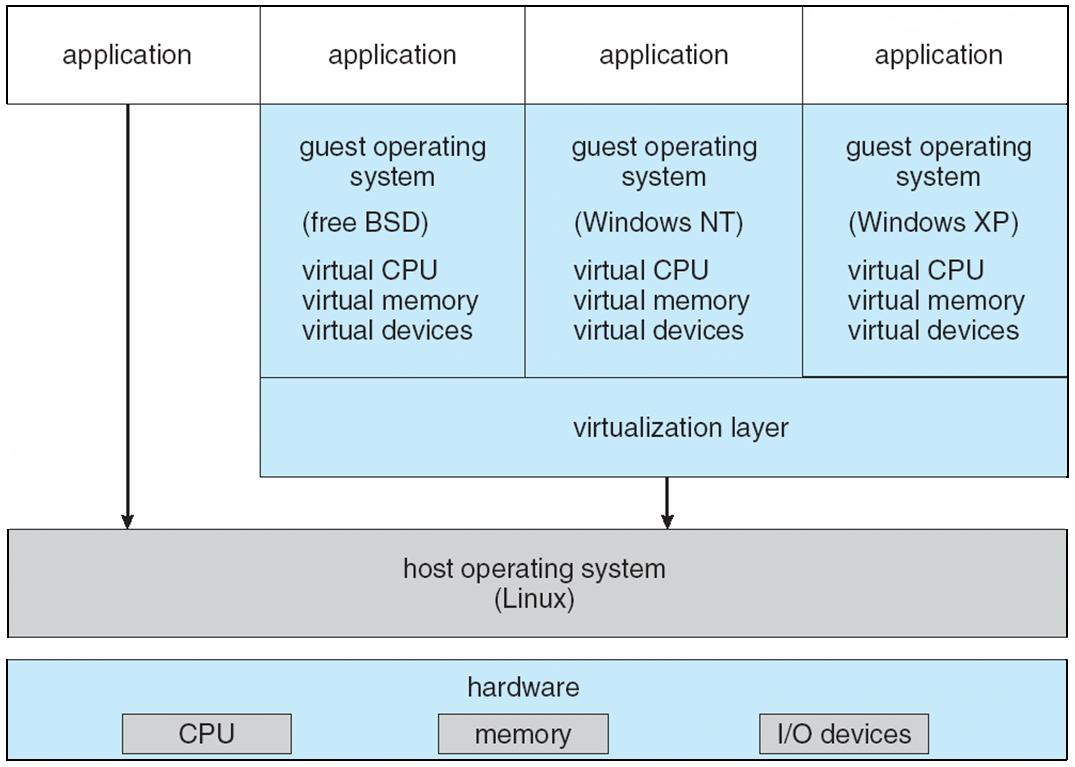
\includegraphics[scale=0.35] {vmwarearchi.png}
		\\
		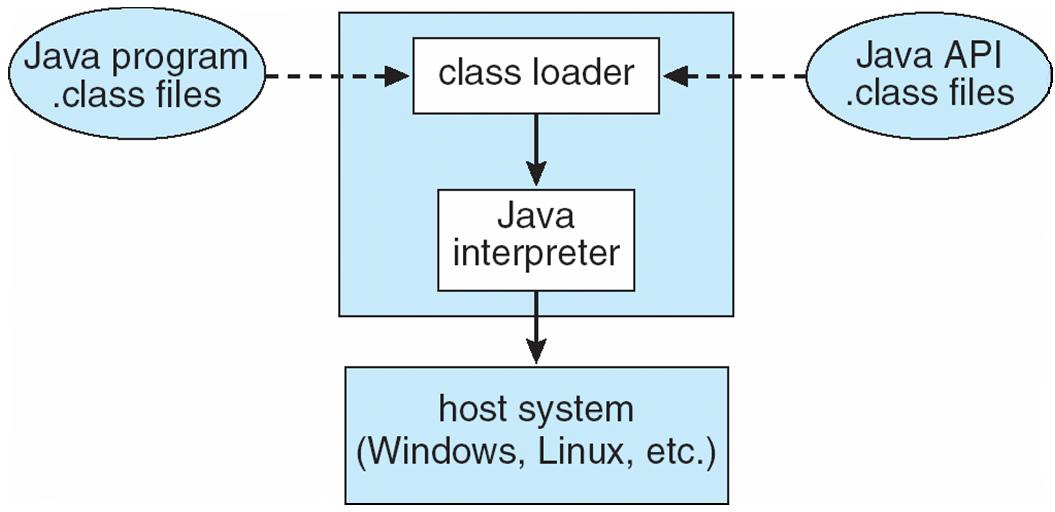
\includegraphics[scale=0.3] {javavm.png}
	\end{center}


\chapter{03aProcess-management}
\chapter{03bProcess-management-scheduling}
\chapter{04Process-coordination}
\chapter{05aMemoryManagement}
\chapter{05bMemoryManagement}
\chapter{05cMemoryManagement}
\chapter{06aFileSystems}
\chapter{06bFileSystems}
\chapter{07aImplementingFileSystems}
\chapter{07bImplementingFileSystems}
\chapter{08SecondaryStorageStructure}
\chapter{09IoSystems}

\end{document}
